\section{利用GDB跟踪getpid系统调用}

NPUcore的系统调用是基于中断来实现的,大致会经历以下步骤,如\autoref{table:系统调用通用过程}:
(用户态,内核态由CPU特定寄存器中的几位来表示)

\begin{table}[h]
    \centering
    \caption{系统调用通用过程}
    \label{table:系统调用通用过程}
    \begin{tabular}{|c|c|}
        \hline
        \textbf{内核态}  & \textbf{用户态}     \\\hline
                        & 执行ecall          \\\hline
        硬件断点保存     &                    \\\hline
        OS手动断点保存   &                    \\\hline
        中断处理         &                    \\\hline
        中断返回,OS手动断点恢复 &                \\\hline
        ret 硬件断点恢复 &                    \\\hline
                        & 用户程序继续执行     \\\hline
    \end{tabular}
\end{table}

下面请你自己动手,使用调试软件跟踪一遍系统调用。

启动调试后,在sys_getpid函数处打断点,使用命令\lstinline`b sys_getpid`,
如\autoref{fig:在sys getpid函数处打断点}。

\begin{figure}[htb]
    \centering
    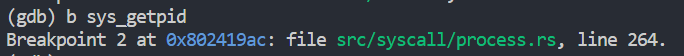
\includegraphics[width=0.8\textwidth]{figures/03-02-利用GDB跟踪getpid系统调用1.png}
    \caption{在sys_getpid函数处打断点}
    \label{fig:在sys getpid函数处打断点}
\end{figure}

输入命令\lstinline`c`,运行程序至断点处,如\autoref{fig:运行程序至断点处}。

\begin{figure}[htb]
    \centering
    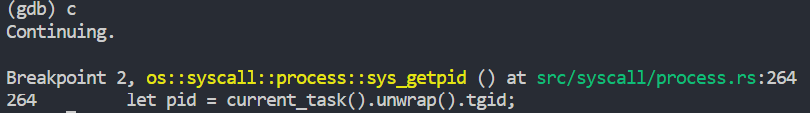
\includegraphics[width=0.8\textwidth]{figures/03-02-利用GDB跟踪getpid系统调用2.png}
    \caption{运行程序至断点处}
    \label{fig:运行程序至断点处}
\end{figure}

此时,程序会陷入内核,在sys_getpid函数处停下。内核的输出如\autoref{fig:断点处内核输出}。

\begin{figure}[htb]
    \centering
    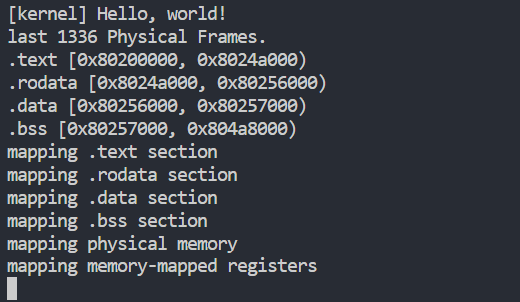
\includegraphics[width=0.6\textwidth]{figures/03-02-利用GDB跟踪getpid系统调用3.png}
    \caption{断点处内核输出}
    \label{fig:断点处内核输出}
\end{figure}


输入命令\lstinline`c`,继续让内核运行。
因为在bash应用程序启动中会多次调用sys_getpid,所以会多次停留在sys_getpid,
如\autoref{fig:多次停在sys getpid}。

\begin{figure}[htb]
    \centering
    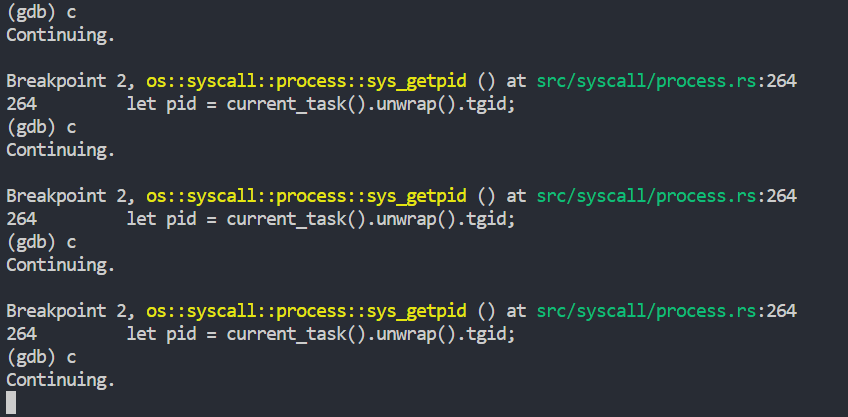
\includegraphics[width=0.6\textwidth]{figures/03-02-利用GDB跟踪getpid系统调用4.png}
    \caption{多次停在sys_getpid}
    \label{fig:多次停在sys getpid}
\end{figure}

最终bash应用完全启动,界面如\autoref{fig:bash界面}。

\begin{figure}[htb]
    \centering
    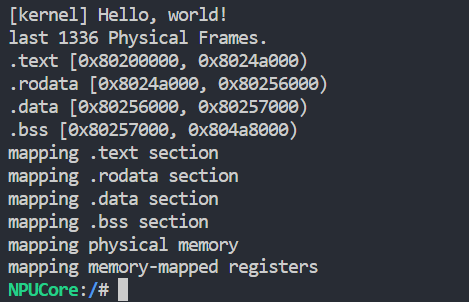
\includegraphics[width=0.6\textwidth]{figures/03-02-利用GDB跟踪getpid系统调用5.png}
    \caption{bash界面}
    \label{fig:bash界面}
\end{figure}